\documentclass[sigconf]{acmart}

\usepackage{geometry}                		
\geometry{letterpaper}                   		                		
\usepackage[parfill]{parskip}    		
\usepackage{graphicx}
\usepackage{subfig}
\usepackage{float}
\usepackage{color}
\usepackage{amssymb}
\usepackage{amsfonts}
\usepackage{amsmath}

\usepackage[framed, useliterate]{mcode}
\usepackage{listings} % For displaying code
\usepackage{algorithm}
\usepackage{algorithmic}
\usepackage{hyperref}

\acmISBN{}
\acmDOI{} 
\setcopyright{none}
\settopmatter{printacmref=false, printccs=false, printfolios=true}

\title{HiggsTweet: Analyzing Influence Propagation During a Viral Event on Twitter}

\author{Kristian Flatheim Jensen}
\affiliation{%
\institution{Norwegian University of Science and Technology}
}

\author{Gudbrand Tandberg}
\affiliation{%
\institution{The University of British Colombia}
}

\begin{document}
\maketitle

\begin{abstract}
In this project we analyze the influence dynamics within a subset of physics-interested Twitter users before, during and after the 4th July 2012 discovery of the Higgs boson, made by researchers at CERN in Switzerland. We study a dataset consisting of a 450k-user Twitter follower network together with a 500k line event log, collected between the 1st and the 7th of July 2012. We use the event log to calculate influence probabilities between pairs of users, these weights are then used to run simulations of Independent Cascade (IC) diffusion processes and to compute near-optimal seed sets using a greedy algorithm. We experiment with several different preprocessing steps and heuristics for reducing the size and runtime of the simulation and optimization steps, and compare seed-sets and expected user influence across our experiments. 
\end{abstract}

\section{Introduction}

Analyzing the spread of information through a large and complex social network is a difficult and interesting problem. In the last 10 years, the Big Data revolution has been driven, to a large extent, by innovations in understanding how humans interact and live in a mobile world. At least some of this progress has been made thanks to inter-disciplinary efforts by researchers in sociology, psychographics, epidemiology, and computer science into understanding the dynamics of social interactions. Already it has become clear the immense opportunities and dramatic shifts this revolution has brought about for marketers, news agencies, individuals and more. We will see in the near dystopian future how the study of social networks will in fact be key to developing political theory (and practice) into the 21st century.

The main goal of the broader research agenda we are following is the open-ended and general question of analyzing the power and influence dynamics of a web-community before, during, and after some major event. This study of course has a much narrower scope. Our lower level goals for this project are twofold, first, we wanted to get hands-on experience with some of the material we covered in class, notably Influence Maximization (IM), second, we wanted to perform an as-complete-as-possible scientific exposition of a new and interesting dataset. We will see how successful we were at the end!

Some questions that guided our efforts were
\begin{itemize}
\item \emph{Which users in the network should we influence, and when should we influence, if we want to spread a rumor during a viral event?}

\item \emph{How do the power dynamics, as computed from an event log change over time during a viral event?}

\item \emph{What does the typical and the atypical user look like, in terms of event history, during a viral event?}

\item \emph{Do the seed-sets (as computed using IM) differ significantly from time to time, or is there overlap?}

\item \emph{To what extent can the selection of seed sets be simplified, or substituted for other statistics- or feature-based heuristics? }

\end{itemize}

\section{Preliminaries \& Related Work}

Network diffusion processes have a long history of study in the social sciences. Some of the early applications include modeling the adoption of new products and technologies, modeling disease outbreaks and word-of-mouth events, and understanding human social dynamics. With the relatively recent advent of global social network platforms such as Facebook and Twitter, many new lines of research in computer science have emerged. In particular, the process of influence propagation in social networks has received a lot of attention.

In the age of Youtube, Facebook and Twitter, the appeal of viral marketing is to many the ultimate free lunch: pick some small number of people to "seed" your idea, get it to "go viral", and watch while it relentlessly spreads to reach millions, all on a shoestring budget. In \cite{watts2007viral}, the authors propose a new model called "Big Seed Marketing" that combines the power of traditional advertising and the extra punch provided by viral propagation. This follows from years on marketing research, see for example \cite{domingos2001mining} for an early study in computing the "value" of a user in a social network. 

The problem of selecting a set of seed-users that will trigger a large cascade of activity was first introduced in \cite{kempe2003maximizing}. In this seminal work the computational problem of maximizing the expected spread of a seed set is formulated as a discrete optimization problem, proven to be NP-hard, and a greedy algorithm with provable approximation guarantees is presented for a class of diffusion models. Importantly, they find that they are able to attain significantly higher values of expected spread by solving the Influence Maximization (IM) problem, as opposed to both random and centrality-based seed-selection methods. Since the greedy algorithm can be relatively slow to run on large networks, several methods have been presented to deal more efficiently with IM. These include the optimized algorithms CELF, MIA, TIM and IMM, \cite{chen2009efficient}, \cite{chen2010scalable}, \cite{tang2014influence}, \cite{tang2015influence}. 

Algorithms for solving the the IM problem all depend on a directed, weighted social network as input. The weight of a directed edge between two users is supposed to represent the degree of influence the one has over the other. Estimating this number is an interesting and general question in itself, and there is still plenty of room for more research here. The problem of estimating influence probabilities was first presented in \cite{goyal2010learning}, where the authors present static and time-dependent models for learning influence weights from a log of events. 

The related question of identifying influential spreaders in complex networks was partly answered in \cite{kitsak2010identification}. In it, they find that there are circumstances where the best spreaders do not correspond to the best connected people or to the most central people (high betweenness centrality), rather, they are located within the core of the network as identified by the $k$-shell decomposition, and that when multiple spreaders are considered simultaneously, the distance between them becomes the crucial parameter that determines the extent of the spreading. More answers to the same question came in \cite{bakshy2011everyone}, where the authors investigate the attributes and relative influence of a large Twitter follower graph over a two month interval in 2009. They find that the largest cascades tend to be generated by users who have been influential in the past and who have a large number of followers. They also find that hashtags that were rated more interesting and/or elicited more positive feelings were more likely to spread. They also find that predictions of which particular user will generate large cascades are relatively unreliable. For a survey of computational models of influence propagation, see e.g. \cite{bonchi2011influence}, or \cite{gomez2012inferring}.

In \cite{wang2010community}, the authors present a community-based algorithm for mining top-$k$ influential nodes in social networks. Their method is found to lead to a decrease in runtime, while not sacrificing much in terms of spread. This is perhaps not so surprising, given the above result that distance between seed-users becomes the crucial parameter that determines the extent of the spreading. 

Combining the problems of influence maximization, influence estimation, and viral event dynamics, we are faced with the problem of real-time IM on dynamic social networks. This has been addressed in \cite{rodriguez2012influence}, and more recently in \cite{wang2017real}.

Some other relevant and recent research that we have taken inspiration from include studies of differences in mechanics of diffusion across topics \cite{romero2011differences}, the dynamics of protest recruitment \cite{gonzalez2011dynamics}, sentiment reciprocality in reply networks \cite{bliss2012twitter} and prediction of social-link creation times \cite{meeder2011we}.

The Higgs dataset was first presented in \cite{de2013anatomy}, where the authors present the dataset, explore the spatio-temporal properties of the data, and demonstrate a model for the information spreading in the social network during the event.

\section{The Data Set}

The dataset we are working with consists of a social network and an action log. The social network contains just over 450k unique Twitter users with just over 14.8M directed edges representing one user following another. The action log is a list of 563069 events of the form 

\begin{center}
\begin{verbatim}
            user1, user2, event_type, time
\end{verbatim}
\end{center}

where \verb+user1+ is the user who performs the action, \verb+user2+ is the user to whom the action is directed, \verb+event_type+ is one of either RT (retweet), MT (mention) or RE (reply), and \verb+time+ is the UNIX timestamp for the event. The dataset was scraped from the web using the Twitter API by the authors of \cite{de2013anatomy}. The contents of the tweets and the identity of the tweeters is, unfortunately, not available. All we do know is that all of the tweets corresponding to events in the log contained one or more of the hashtags "LHC", "Higgs", "CERN", and "boson". It would have been very interesting to have access to not only the contents of the tweets, e.g. in order to perform some sort of semantic analysis, but also to have access to standalone tweets in the period, not just user to user interactions. 

Of all the events in the log, roughly 62\% of them are between two users where at least one of the users follows the other. This means that roughly 38\% of the events are directed between "complete strangers". Out of all the events, 63\% are retweets, 30\% are mentions, and 7\% are replies. 

The authors of \cite{de2013anatomy} identify four different periods into which the events can be divided:

\begin{description}
\item[Period I] Before the 2nd July, there were some rumors about the discovery of a Higgs-like boson at the Tevatron accelerator
\item[Period II] On the 2nd July at 1PM GMT, scientists at the Tevatron accelerator in Fermilabs, Illinois, announced that they had discovered the Higgs boson with a 1 in 550 likelihood. 
\item[Period III] After 2nd July and before 4th July there were many rumours about the Higgs boson discovery at the LHC. 
\item[Period IV] The main event was the announcement on 4th July at 8AM GMT by the scientists at CERN. After 4th July, popular media covered the event. 
\end{description}

The distribution of events in the four periods are described in \autoref{tweetsperhour} and \autoref{activityperiod}. As we can see from this distribution there is not much activity in the first periods, which is understandable considering the rumours were in an early phase. In this paper we will thus divide the activity into two periods.

\begin{description}
\item[Period I] Rumour phase. This is the combination of period I, II and III above.
\item[Period II] Post-release (eh, har du ett smoothere navn #gubbis?). This is period IV above.
\end{description}


\begin{figure}[htbp]
\begin{center}
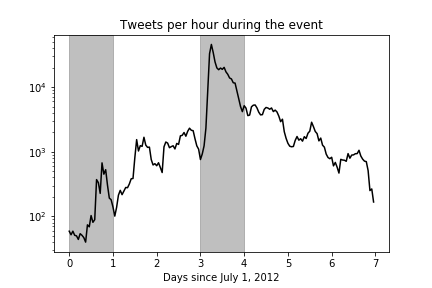
\includegraphics[width=\linewidth]{Figures/tweetsperhour.png}
\caption{Activity levels through time during the event.}
\label{tweetsperhour}
\end{center}
\end{figure}

\begin{table}[htp]
\caption{Distribution of activities in the different periods.}
\begin{center}
\begin{tabular}{|c|c|}
\hline
 Period & \#activities \\
\hline
 I      & 4170  \\
 II    & 3720   \\    
 III   & 171196   \\   
 IV &   383983 \\
 \hline
\end{tabular}
\end{center}
\label{activityperiod}
\end{table}

For completeness, the distribution of in- and out-degrees of each user (number of followers and following, respectively) can be seen in \autoref{deg}, and the average values of the same quantities in \autoref{following}

\begin{figure}[htbp]
\begin{center}
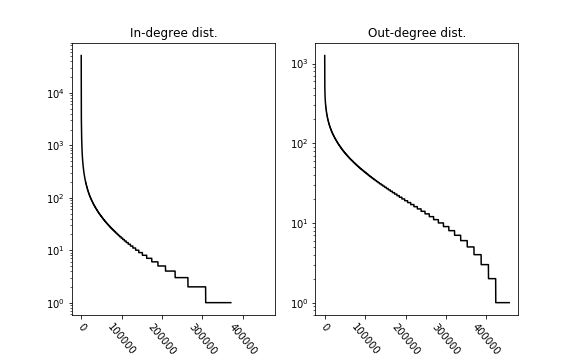
\includegraphics[width=\linewidth]{Figures/deg.png}
\caption{Distribution of in- and out- degree of users in the social network}
\label{deg}
\end{center}
\end{figure}

\begin{table}[htp]
\caption{Average number of followers/following in the social network}
\begin{center}
\begin{tabular}{|c|c|c|}
\hline
 & \#followers & \#following \\
 \hline
mean &32.5 & 32.5 \\
median & 4.0 & 16.0 \\
\hline
\end{tabular}
\end{center}
\label{following}
\end{table}

\section{Our Approach}

\subsection{Computing Influence Probabilities}

In this paper, our goal is to experiment with IM on the Higgs dataset presented above in order to answer some of the questions stated in the introduction. In order to do this, we first combine the social network and the action log into a hybrid multi-digraph as follows: every node in the social network is first added to the hybrid network. Then, every link in the social network is added as a link in the hybrid network with the label "FR". Finally, all events in the action log are added as links in the hybrid network labelled as either "RT", "MT", or "RE". Later, we will also experiment with creating these graphs on a per-period level, so as to compare seeds over time.

The next step is to convert the hybrid multi-digraph into a weighted digraph, where, hopefully, the weights in the graph correspond roughly to the level of influence one user exerts over the other. This digraph can then be used to run IM experiments. \autoref{multidigraph} shows the process schematically in a simple setting. 

\begin{figure}[htbp]
\begin{center}
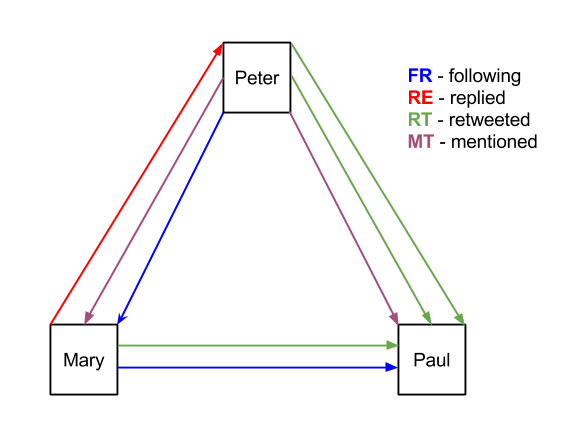
\includegraphics[width=.5\linewidth]{Figures/MultiDiGraph.png}
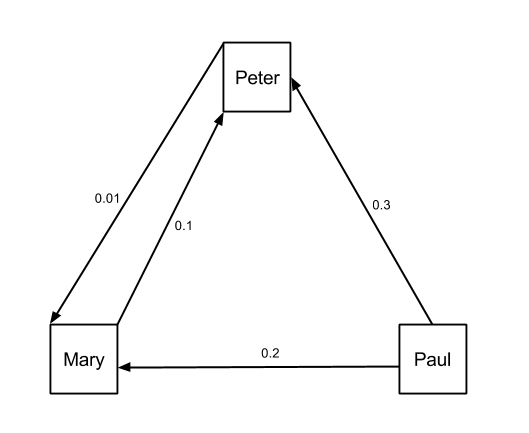
\includegraphics[width=.45\linewidth]{Figures/MultiDiGraphII.png}
\caption{\emph{Left:} original hybrid unweighted multi-digraph
\emph{Right: } influence-weighted digraph}
\label{multidigraph}
\end{center}
\end{figure}

As mentioned earlier, there are many viable ways of estimating the weights in the digraph. We propose a simple additive-weights method, where all parallel edges in the network are combined using predetermined weights per type, with \hspace{0.02cm}$\mathcal{W} = \{w_{\text{FR}}, w_{\text{RT}}, w_{\text{MT}}, w_{\text{RE}}\}$.

\begin{equation}
p_{uv} = \min \left\{1, 
h\left(\sum_{e = (v, u, t)}w_t\right) \right\},
\end{equation}

where the sum ranges over all edges $e$ from $v$ to $u$ with type $t$. We find this method to be simple, cheap and effective, but it is hard to validate whether our formula actually captures the relative influence levels present in the user-set. We set the weights in $\mathcal{W}$ using a combination of trial and error and relative frequency of action-types in the event-log. An advantage of our weights-method is that we can simply choose to set $w_{\text{FR}} = 0$, which means the resulting digraph has roughly 15M fewer edges, drastically decreasing the runtime of our algorithms, as we will see later. 

It is an interesting question whether the weights can be set in a more principled manner, and we leave this for later work. However the weights $p_{uv}$ are computed, it is evident that they are paramount to the later success of our IM campaign. Given a set of weights, it is hard to validate their accuracy without expensive and intrusive user-surveys, or access to extensive event-logs. Furthermore, the weight's impact on both the diffusion process and the runtime of the algorithm is significant. For these reasons we stick to our simple formula for the remainder of this paper. The distribution of influence weights in the network can be seen in \autoref{puv_dist}. 

\begin{figure}[htbp]
\begin{center}
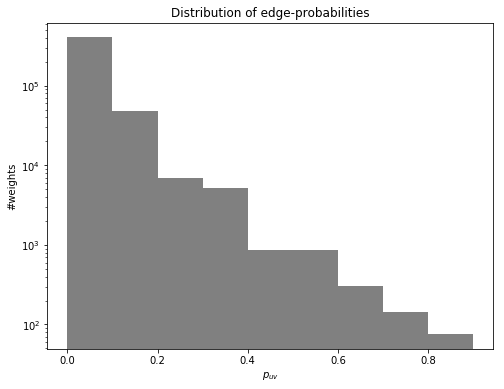
\includegraphics[width=\linewidth]{Figures/puv_dist.png}
\caption{Distribution of edge-weights in the social/action hybrid network}
\label{puv_dist}
\end{center}
\end{figure}

\subsection{Influence Maximization}

Suppose we are an evil galactic empire, and due to universe-threatening circumstances we need to shut down research in particle physics on planet earth. But we are very far away from planet earth, and the only way to do this is to monitor the radio signals in space. Under these circumstances, one way to "shut down"\footnote{Stop, hinder, end, obliterate, assassinate, etc.}the particle physics community would be to infiltrate their twitter feed and manipulate them in some way. 

We hope to make some progress towards an effective solution to this problem in this paper. However, we are not an evil galactic empire..

The aim of Influence Maximization (IM), is to "activate" a large number of users in a social network $G = (V, E, p_{uv})$, by activating a smaller number of seed-users, $S$. Given any discrete diffusion process on a social network and a seed set $S$ denote the sets $S = A_0, A_1, \dots, A_n, \dots$ as the sets of active users at each timestep $0 \leq n \leq \infty$. Assuming it exists, denote the terminal state of the diffusion process by $\Phi(S) \subseteq V$. We define the \emph{expected spread} of a seed set $S$ as

\begin{equation}
\sigma(S) = \mathbb{E}\left[ |\Phi(S)| \right],
\end{equation}

and our goal is to maximize this function over all seed sets subject to a cost constraint. In our experiments, we employ the Independent Cascade (IC) diffusion model which works as follows: we start with an initial set of active nodes $A_0$, and the process unfolds in discrete steps according to the following randomized rule. When node $u$ first becomes active in step $t$, it is given a single chance to activate each currently inactive neighbor $v$; it succeeds with a probability $p_{uv}$ (If $v$ has multiple newly activated neighbors, their attempts are sequenced in an arbitrary order.) If $u$ succeeds, then $v$ will become active in step $t + 1$. The process terminates when no more activations are possible.

The IC model is one of the conceptually simplest diffusion models, based on work in interacting particle systems. A particular useful property of the model is that the corresponding expected spread function $\sigma$ is monotone and submodular. This means we can use a greedy algorithm to achieve a $(1 - 1/e)$-approximation to the optimal solution. However, since the greedy algorithm needs to compute the marginal gain of adding every node in the network to the seed set at each time step, the runtime of the basic greedy algorithm is simply prohibitive for networks of the size we are working with. For this reason we chose to use the Cost Effective Lazy Forwarding (CELF) algorithm, which has a significant speedup in runtime at no sacrifice in approximation guarantee. Even so, the runtime of running a complete IM trial is quite high on our dataset. Most of the time is spent in a subprocedure that runs Monte Carlo simulations to approximate the expected spread of a seed set. It has been the main focus of our project to experiment with heuristics, alternatives, and optimizations for running a full greedy optimization on a large network, without resorting to algorithms that sacrifice another $\epsilon$ on the approximation guarantee, such as MIA and TIM.

\section{Results} 

\section{Discussion}

\subsection{Future Work}

In this paper we have only just started learning about influence dynamics on social networks. We have touched upon many interesting, difficult, and open questions in this line of research. 

Continuous time models, 

Content of tweets - sentiment analysis. 

Compute $p_{uv}$ using unsupervised learning approach. Perform evaluative analysis. 

\section*{TODO FREMOVER}
\begin{enumerate}
\item Decide on graphs, generate graphs
\item Decide on seed sets, generate seed sets
\item Set up and run IM experiments (on UBC cluster?)
\item Plot \& write about the results
\end{enumerate}

\nocite{*}
\bibliography{bibliography.bib}
\bibliographystyle{plain}

\end{document} 
